\documentclass{beamer}

\usepackage{amsmath}

\usetheme{AnnArbor}
\usecolortheme{crane}
\usefonttheme[onlymath]{serif}

\title{Deep Learning - Foundations and Concepts}
\subtitle{Chapter 18. Normalizing Flows}
\author{nonlineark@github}
\date{\today}

\begin{document}

\begin{frame}
    \titlepage
\end{frame}

\begin{frame}
    \frametitle{Outline}
    \tableofcontents
\end{frame}

\begin{frame}
    \frametitle{Normalizing flows}
    \begin{itemize}
        \item We define a distribution $p_{z}(z)$ over a latent variable $z$.
        \item And we use a deep neural network architecture to define an invertible function $x=f(z;w)$ that transforms the latent space into the data space.
        \item We can ensure that the overall function is invertible if we make each layer of the network invertible:
        \begin{itemize}
            \item $x=f^{A}(f^{B}(f^{C}(z)))$.
            \item $z=g^{C}(g^{B}(g^{A}(x)))$.
        \end{itemize}
    \end{itemize}
\end{frame}

\begin{frame}
    \frametitle{Normalizing flows}
    This approach to modelling a flexible distribution is called a normalizing flow because:
    \begin{itemize}
        \item The transformation of a probability distribution through a sequence of mappings is somewhat analogous to the flow of a fluid.
        \item The effect of the inverse mapping is to transform the complex data distribution into a normalized form, typically a Gaussian distribution.
    \end{itemize}
\end{frame}

\section{Coupling Flows}

\begin{frame}
    \frametitle{Real NVP}
    \begin{figure}
        \caption{A single layer of the real NVP normalizing flow model}
        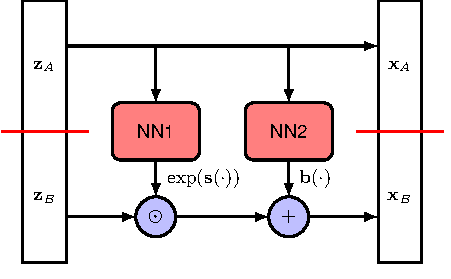
\includegraphics{Figure_1.pdf}
    \end{figure}
\end{frame}

\begin{frame}
    \frametitle{Real NVP}
    Real-valued non-volume-preserving (real NVP) partitions the latent variable $z\in\mathbb{R}^{D}$ and the output vector $x\in\mathbb{R}^{D}$ into two parts: $z=(z_{A},z_{B})$ and $x=(x_{A},x_{B})$, where $z_{A},x_{A}\in\mathbb{R}^{d}$. The transformation function is given by:
    \begin{align*}
        x_{A}&=z_{A} \\
        x_{B}&=\exp(s(z_{A};w))\odot{}z_{B}+b(z_{A};w)
    \end{align*}
    where $s(z_{A};w)$ and $b(z_{A};w)$ are the real-valued outputs of neural networks, and $\odot$ denotes element-wise multiplication of the two vectors.
\end{frame}

\begin{frame}
    \frametitle{Real NVP}
    The overall transformation is easily invertible:
    \begin{align*}
        z_{A}&=x_{A} \\
        z_{B}&=\exp(-s(x_{A};w))\odot(x_{B}-b(x_{A};w))
    \end{align*}
    The Jacobian matrix of this inverse mapping is given by:
    \begin{equation*}
        J=\begin{pmatrix}
            I_{d}&0 \\
            \frac{\partial{}z_{B}}{\partial{}x_{A}}&\mathrm{diag}(\exp(-s(x_{A};w)))
        \end{pmatrix}
    \end{equation*}
    We see that the Jacobian matrix is a lower triangular matrix, and its determinant is simply given by the product of the elements of $\exp(-s(x_{A};w))$.
\end{frame}

\begin{frame}
    \frametitle{Real NVP}
    \begin{figure}
        \caption{A double-layer structure where the roles of $z_{A}$ and $z_{B}$ are reversed in the second layer}
        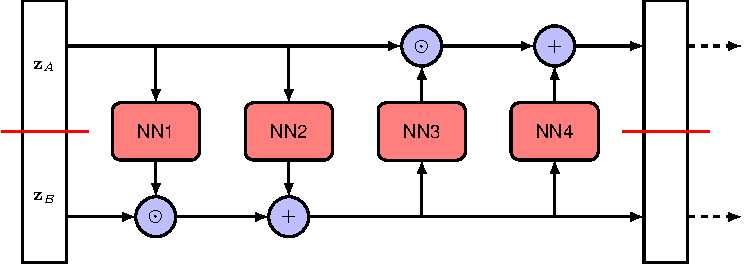
\includegraphics[width=0.8\textwidth]{Figure_2.pdf}
    \end{figure}
\end{frame}

\begin{frame}
    \frametitle{Coupling flows}
    The real NVP model belongs to a broad class of normalizing flows called coupling flows:
    \begin{align*}
        x_{A}&=z_{A} \\
        x_{B}&=h(z_{B},g(z_{A};w))
    \end{align*}
    where:
    \begin{itemize}
        \item $h(z_{B},g)$ is a function of $z_{B}$ that is efficiently invertible for any given value of $g$ and is called the coupling function.
        \item The function $g(z_{A};w)$ is called a conditioner and is typically represented by a neural network.
    \end{itemize}
\end{frame}

\end{document}